\documentclass[main.tex]{subfiles}

\begin{document}
\chapter{Benchmarking}
\chaplabel{benchmarking}
Military and commercially available mine detection vehicles were assessed to give insight into what platforms are currently being used. This gave a basis for the minimum requirements to be set for the project and to understand what challenges would need to be overcome.

\section{Remotely Controlled Platforms for Landmine Detection}
The use of a vehicle for landmine detection allows for larger areas to be scanned in a shorter period of time. Vehicles can also support greater loads than any human operator can, which means that more sensing equipment can be carried; this in turn increases sensing capability, and reduces the likelihood of false positives. If the vehicle can operate remotely or autonomously, the risk to human operators can be eliminated entirely. For these reasons, remotely controlled or autonomous platforms have become a popular tool for landmine detection. This section looks a number of such platforms that are currently in operation or in development. 

%\subsection{Landmine detection vehicles}

In military scenarios, the key priority is to clear a path as quickly as possible for a convoy \parencite{portugal2014}. In many cases, landmine detection is coupled with landmine clearance. On the other hand, humanitarian demining requires greater levels of accuracy and effort. A clearance rate of 80\% is generally accepted in combat, a figure which only needs to apply to pathways where troops or convoys will travel; for humanitarian situations, the area required to be cleared is much larger, and such a low clearance is not accepted \parencite{habib2008}.  

\begin{figure}[ht]
\centerline{
\begin{tabular}{cc}
\subfloat[FORESIGHT RDV \parencite{canada2004}]{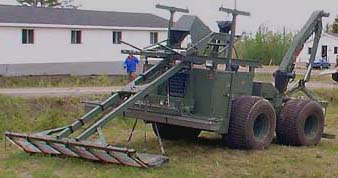
\includegraphics[height=0.25\textwidth]{2-Benchmarking/foresight.jpg}}
& \subfloat[NIITEK Minestalker \parencite{niitek2015}]{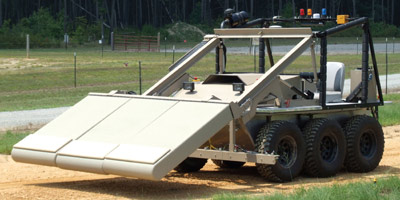
\includegraphics[height=0.25\textwidth]{2-Benchmarking/minestalker.jpg}} \\
\end{tabular}}
\caption{Military and commercially available vehicles for landmine detection}
\figlabel{military}
\end{figure}
 
\Figref{military} shows two types of remotely controlled or autonomous landmine detection vehicles that have been used in military operations or are commercially available for humanitarian demining. 

\paragraph{General Dynamics FORESIGHT RDV} FORESIGHT is a multi-sensor landmine detection system, mounted on a vehicle that can be controlled remotely. The vehicle usually travels with a protection vehicle, which clears the the path ahead of surface-based devices, as well as mines just below the surface \parencite{canada2004}. The sensor suite consists of four independent systems, the data from which is fused to accurately detect a range of threats. At a minimum a metal detector array which is 3 m wide is used for the detection of metallic parts, even when the metal content is low. The 3 m GPR array with ultra-wide band capabilities (1-3 GHz) can detect larger mines at up to 30 cm below the soil surface. An infra-red camera with 8-14 micrometre wavelength is used to detect changes in soil density which occur when mines are buried \parencite{canada2004}. Finally, a thermal neutron activation detector directly detect explosives through measurements of the soil nitrogen level; this provides an added level of target confirmation \parencite{general2009}. The sensor suite can operate at a forwards speed of 3-4 km/h, and in the event that a detection is made with a sufficient confidence level, the onboard marking system is used to physically mark the threat location \parencite{canada2004}.

\paragraph{NIITEK Minestalker} Developed by the US Department of Defense and NIITEK for humanitarian demining, the Minestalker system was built to detect anti-tank mines at depths greater than 5 to 10 cm \parencite{laudato2014}. The system utilises a high performance 3.2 m VISOR GPR array and optional 3 m See-Deep metal detector array \parencite{niitek2015}. The sensors are mounted on a tractor vehicle which can be controlled remotely; the accompanying software system ensures that there is a high detection probability and a low number of false alarms. The system is a "user in the loop system", in the sense that the vehicle stops when a target is detected and waits for further instructions \parencite{laudato2014}. Targets are marked both physically and with GPS, with a 1 metre resolution. The vehicle itself can advance and detect threats in real time at up to 15 km/h \parencite{niitek2015}.

% \subsection{Research Vehicles}
% While commercially available vehicles for landmine detection are often modelled on military vehicles, research vehicles are much more varied in their design (\Figref{research}). These vehicles have been developed by universities or other research organisations, and in most cases have not seen any operational use.

% \begin{figure}[ht]
% \centerline{
% \begin{tabular}{cc}
% \subfloat[Clearpath Husky \parencite{hennessey2014}]{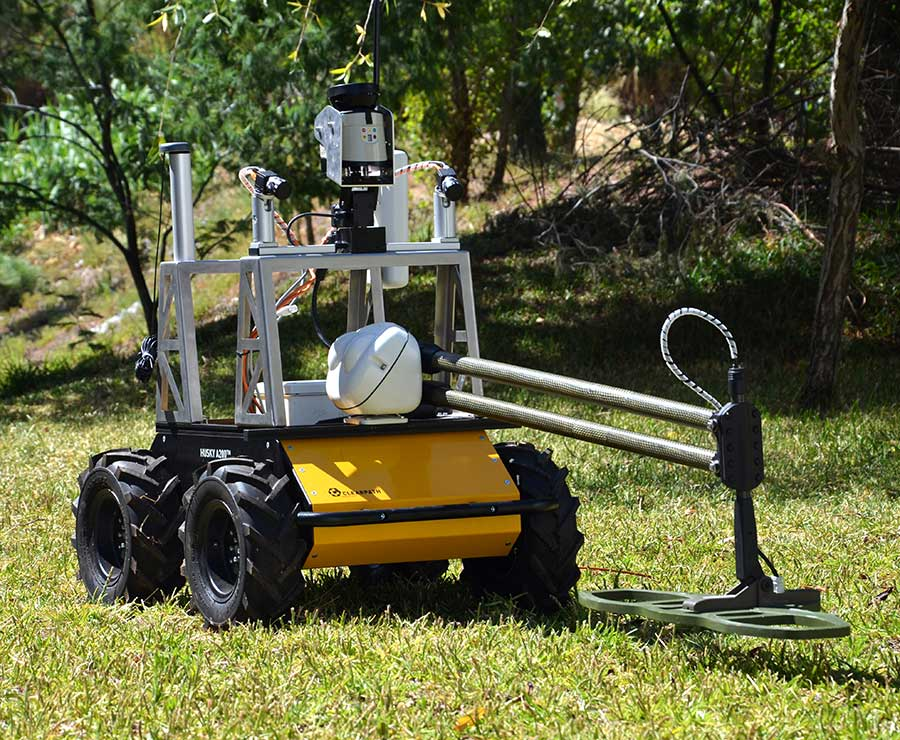
\includegraphics[height=0.3\textwidth]{2-Benchmarking/clearpath.jpg}} 
% & \subfloat[SILO6 \parencite{santos2007}]{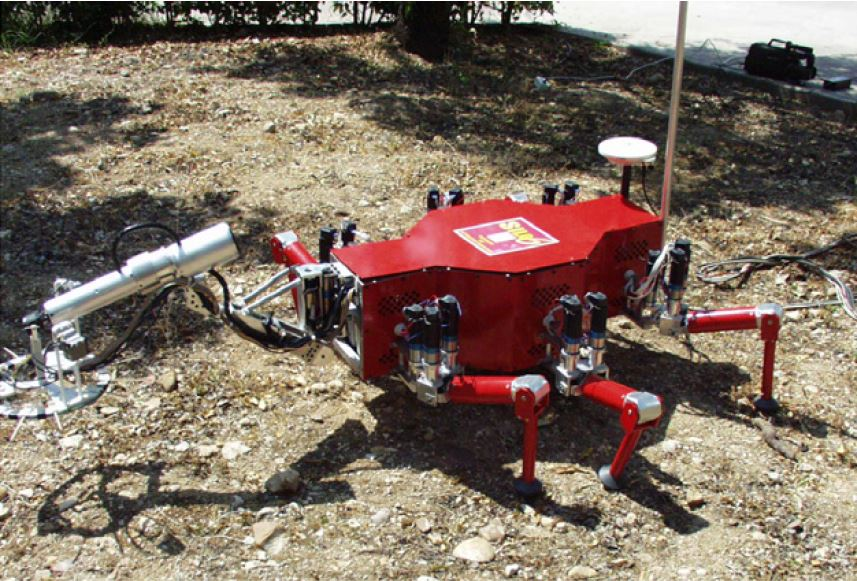
\includegraphics[height=0.3\textwidth]{2-Benchmarking/silo6.jpg}}\\
% \subfloat[tEODor \parencite{cubber2014}]{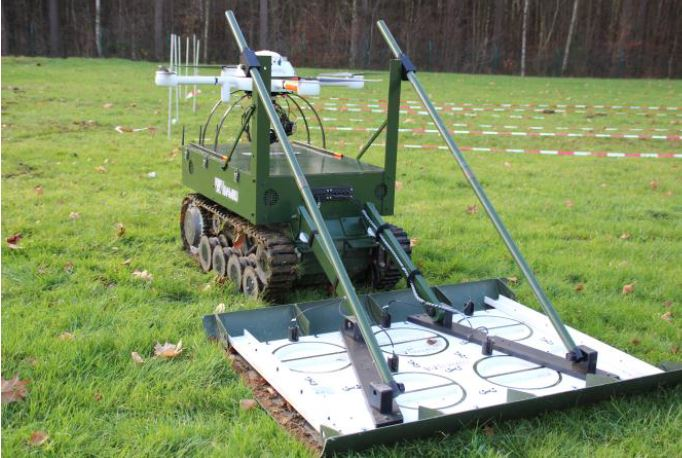
\includegraphics[height=0.3\textwidth]{2-Benchmarking/teodor.jpg}} 
% & \subfloat[Gryphon \parencite{fukushima2008}]{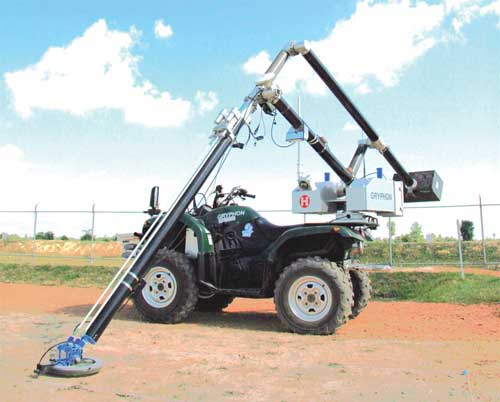
\includegraphics[height=0.3\textwidth]{2-Benchmarking/gryphon.jpg}}
% \end{tabular}}
% \caption{Research vehicles for landmine detection}
% \figlabel{research}
% \end{figure}

% \paragraph{Clearpath Husky} The Husky is an autonomous vehicle produced by Clearpath Robotics. In 2012, a team at the University of Coimbra (Portugal) used this platform as  foundation to create a landmine detection vehicle \parencite{hennessey2014}. The sensor suite consists of a metal detector on a robotic arm, and a GPR. The Husky itself has autonomous capabilities, meaning it can complete a mission without operator interaction \parencite{portugal2014}. The vehicle has an operational speed of 1 m/s, with an operating time, limited due by the battery life of the Husky, of 3 hours. 

% \paragraph{SILO6} SILO6 is a six-legged landmine detection robot. The six legs allow it to better traverse rough terrain, and increase mobility; in order to increase stability, the robot can lower its centre of gravity by bending its legs \parencite{santos2007}. The robot is semi-autonomous, however it has a limited sensor capability. The only sensor currently used is a Schiebel AN-19/2metal detector, which is capable of detecting objects with a low metal content. The design of the platform restricts the operating speed to 0.5 m/s, with a typical speed of 0.1 m/s, while the maximum operating time is 1 hour \parencite{portugal2014}.  

% \paragraph{tEODor} The tEDOor platform is a tracked, remotely controlled vehicle that is commercially available for the disposal of explosive ordnance. The platform was heavily modified by the Royal Military Academy (Belgium) to assist in humanitarian demining \parencite{cubber2014}. A metal detector array is fitted to the front of the platform, which is able to detect both small and large mines. The system works in conjunction with an unmanned aerial vehicle, which firstly scans the area using visual and infra-red sensors, and identifies points of interest which tEODor investigates. Being a tracked vehicle, the operating speed is limited, in this case to a maximum of 0.8 m/s, while the operating time is 203 hours \parencite{portugal2014}.   

% \paragraph{Gryphon}
% The Gryphon project is larger in scale than the rest of the research projects introduced. It uses a commercially available quad bike on which a large arm has been fitted \parencite{fukushima2008}. The length of the arm allows the vehicle to remain completely outside of the test lane, meaning this it is less susceptible to damage. A metal detector or GPR can be fitted to the end of the arm, though not at the same time. Since the platform is a larger vehicle, is can be operated at speeds of up to 5 m/s, and the petrol engine allows a 10 hour operating time \parencite{portugal2014}.  

% The various vehicles introduced show that there are many approaches to automated landmine detection, both in terms of the platforms used and the sensors available. While many solutions exist, no one method can be adapted to all scenarios, and there is much room for innovation and further research. \textcolor{red}{Need to speak about the challenges that are present}

%\section{Landmine Detection}
%There have been similar projects that have used MD, GPR or a  combination of both to achieve detection and classification of landmines or unexploded ordinances (UXO). The various models of MD, GPR will be compared in order to determine if the specific details are suitable for landmine detection and if the scenario of operations (\textcolor{red}{insert reference to scenario of operations}) are achievable based on these specifications. 

% \subsection{Metal Detectors}
% \textcolor{red}{Insert some benchmarking here that Rahul did}

% \subsection{Ground Penetrating Radar}
% \textcolor{red}{Need to relate to the scope as well, i.e. soil types and operational environments\\}
% What has been achieved with the GPR in terms of the operation environment and soil types. etc. that can be linked and based on

%In order to meet the system requirements \textcolor{red}{(insert reference to system requirements here)} and  scenarios of operation of the landmine, there are operating parameters required. The operating specifications of a GPR for landmine detection are listed as follows \textcolor{red}{insert Pasolli reference here}:
% \begin{itemize}
% \item{\textbf{frequency:} 10 MHz - 3 GHz}
% \item{\textbf{Penetration depth:} 1 cm - 3 m.}
% \item{\textbf{Surface types:} Sand, humus soil}
% \item{\textbf{Operating time:} 1 ns to 60 ns}
% \item{\textbf{No. of data scans:} 200 - 600}
% \end{itemize}

%The following comparisons of specific GPRs that may be used in landmine detection should meet or exceed the specifications above. There are various types of commercial GPRs, such as NIITEK, SIRO-Pulse, and others as provided below. %-Still changing this part. 

%\paragraph{NIITEK GPR}
%AS provided in landmi
%\paragraph{SIRO-Pulse}

%\paragraph{DX Antenna Array GPR} This type of GPR meets the operating criteria above as specified in \textcolor{red}{see appendix}. There are various applications that this GPR may be used including archaeology,

%The detection of subsurface objects is one of the main uses for a GPR. This concept may be used in various applications including landmine detection. The GPR is able to detect landmines with various types of casing. An advantage of the GPR sensor is that there are both handheld and array types which assist in both manned and unmanned landmine detection operations. There are two types of GPRs, namely pulse radar (time-domain) and frequency-domain \textcolor{red}{specific reference here}. 

%In order detect and identify the subsurface objects as mentioned in \textcolor{red}{reference objective section}, the GPR signals are required to be processed. There are various methods implemented to detect landmines using GPR \textcolor{red}{INSERT CITE}. The first part is the preprocessing of the signals in order to remove signal clutter. This is processed further in order to identify the object under the surface and minimise false positives.

%The detection and classification of landmines and subsurface objects are achieved through existing algorithms, such as, hough transformation, bayesian, feature extraction, kalman filters.   

%\textcolor{red}{NOTE: Need to mention anything commercialised here. Types of GPR used, and the operation frequency they used. The penetration depth etc. etc. Nothing too specific. Just how they've done it. Elaborate on the types in Literature review.} \textcolor{green}{perfect. this is exactly what i was going to put in here - i had a spreadsheet on the GoogleDrive with most of this data in it, but it seems to have gone walkabout}

% Need to check everything
%NOTE NO PHYSICAL MARKING OF THE LANDMINE
%It is also possible to detect the composition of the explosives used in the landmines, however, this is only used in conjunction with the electromagnetic properties returned to receive the signals. 

%Link to Challenges in identifying the landmine due to background noise etc. 
% Need to mention that a database for identification is generally difficult to achieve with regards to current mines. Limitation include that the objects have similar reflected signals, such as rocks vs composite landmines. 

% Need to talk about the usefulness of the GPR and landmine together. How they complement each other. 

\section{Mine detection equipment capabilities}
Current mine sweeping methods that employ the use of handheld metal detectors achieve high rates of detection for subsurface metallic mines. The main limitations of the handheld metal detecting systems is the inability to detect mines constructed from non-metallic composite materials, and the shallow depth capabilities provided by the metal detector. These systems also have a high rate of false positives due to the inability for an operator to differentiate between mines and shrapnel fragment or other buried metal objects.

Handheld mine detection devices currently used by the ADF for military purposes include the Minelab F3 series. This device is currently used to clear paths for vehicles by tracking the wheelbase and scanning for anti-vehicle mines. It has a sensing depth suitable to allow the detection of almost all anti-vehicle and anti-personnel mines that will pose a threat to an operator, though has the expected high rate of false positives \parencite{minelabF3}. The process for determining which items are suspicious and require excavation and which items are unremarkable shrapnel is required to be undertaken by a skilled operator.
\begin{figure}[ht]
\centerline{
\begin{tabular}{cc}
\subfloat[Minelab F3 \parencite{minelabF3}]{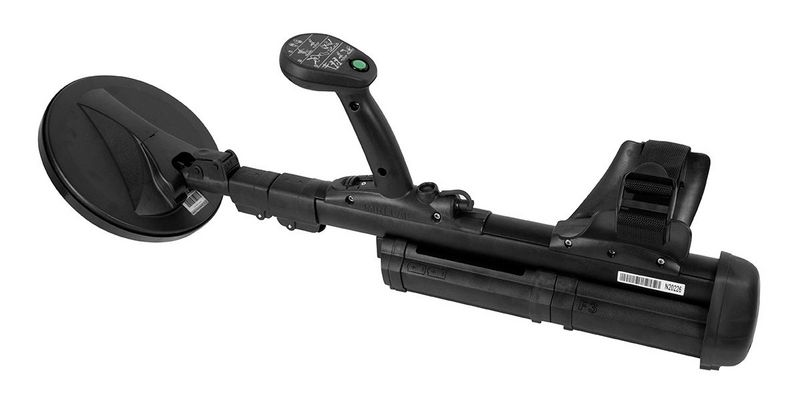
\includegraphics[width=0.5\textwidth]{2-Benchmarking/minelabF3.jpg}} 
& \subfloat[Minelab STMR \parencite{minelabArray}]{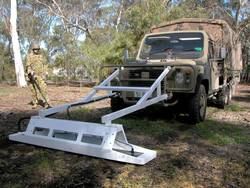
\includegraphics[width=0.4\textwidth]{2-Benchmarking/stmr.jpg}}\\
\end{tabular}}
\caption{Minelab metal detector systems used by the ADF \& DSTG}
\figlabel{metaldetectors}
\end{figure}

Minelab also provides the STMR, a vehicle mounted metal detection array to reduce the need for on-foot operators in front of a convoy. The sensor is capable of sampling at a rate of 200 Hz, meaning that the device is capable of detecting objects while moving at speeds up to 50 km/h \parencite{3dradarDXG}. Like the F3 series, the STMR is capable of detecting minimum-metal mines, such as the composite M14 anti-personnel mine, which contains only a small button sized metal detonator in the entire device \parencite{minelabArray}. The STMR system provides some level of feature recognition, providing a display to the operator inside the vehicle which reports scanned data \parencite{minelabArray}.



Commercially available GPR systems are commonly intended for non-mine detection purposes, such as utility and buried pipe detection. The limitations of 2D radar systems, which include the majority of available GPR devices, is that the narrow scan width means that the antenna is required to pass directly over the mine object to register a detection. A typical scan deviance from the buried object to still consistently register a detection is approximately 150mm \parencite{3dradarDX}.

Commercial 2D GPR systems range from handheld devices which are intended to detect utilities and locate studs in wall cavities, such as the RadioDetection RD8000, have detection depths of only a few centimetres and limited resolution \parencite{rd8000}. More advanced systems with limited depth ranges, such as the US Radar Seeker 2000 HH are capable of detection resolutions to allow identification of a fishing line at depths of 0.6 metres \parencite{usradar}. The ability to consistenty locate features this small are limited by the signal to noise ratio, a property of the soil in which the search is undertaken. Typical limits for detection capabilites of these GPR units range from a few centimetres to many metres in depth, with reduced resolution as depth of scanning increases.
\begin{figure}[ht]
\centerline{
\begin{tabular}{cc}
\subfloat[RadioDetection RD8000 \parencite{rd8000}]{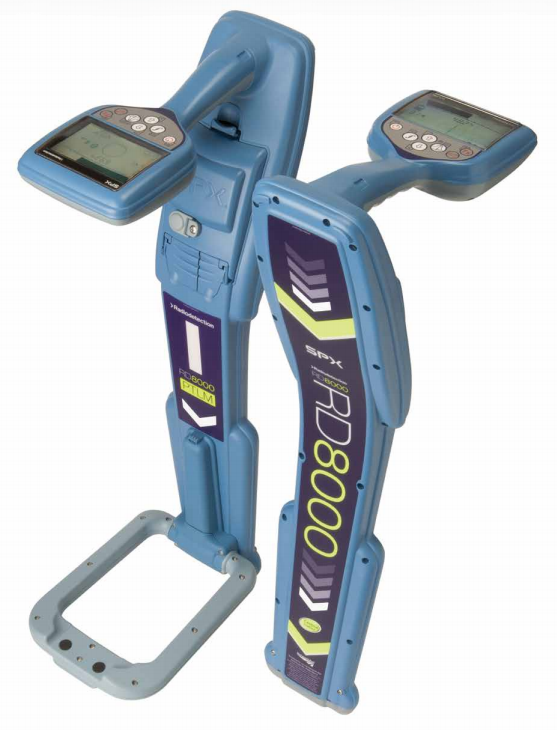
\includegraphics[height=0.5\textwidth]{2-Benchmarking/rd8000.png}} 
& \subfloat[US Radar Seeker 2000 HH \parencite{usradar}]{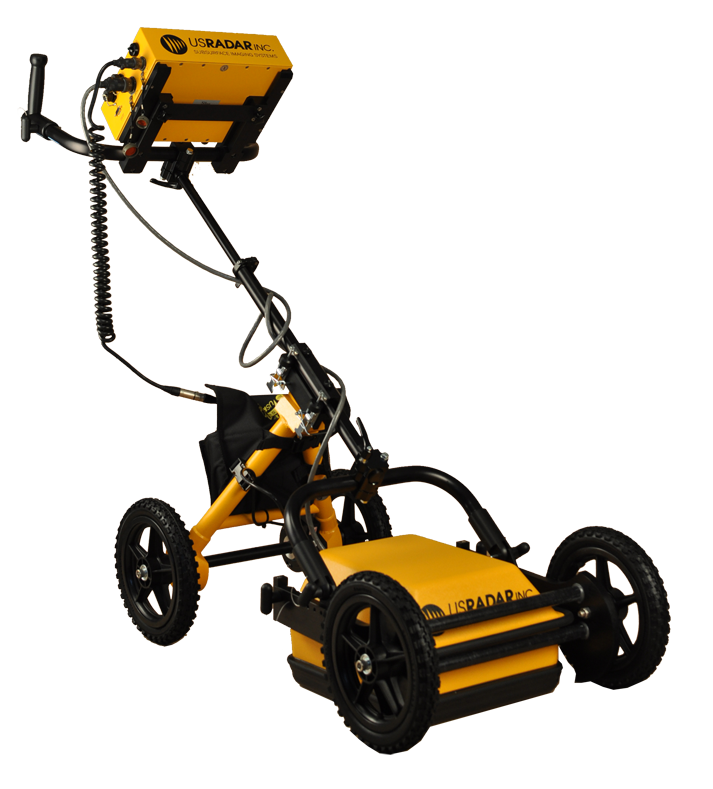
\includegraphics[height=0.5\textwidth]{2-Benchmarking/seeker2000.png}}\\
\end{tabular}}
\caption{Commercially available GPR systems}
\figlabel{cheapradar}
\end{figure}

A common theme among these systems is limited ability for automatic classification of targets. The large majority require a skilled operator to identify all targets and provide no degree of automatic scanning. More advanced and expensive units offer greater software capabilities for data logging and feature identification, though due to their multi-purpose nature are not capable of providing a high degree of mine detection and identification autonomously with software \parencite{rd8000}.



Current state-of-the-art GPR systems for mine detection, such as the DX and DXG series detectors from 3D-RADAR AS have significantly greater detection capacity than other GPR systems. The DX series, which are specially designed for detection of landmines and unexploded ordnance (UXO) is capable of achieving high detection rates (>95\%) of underground mines due to its high resolution. Detection of objects down to 25 mm in feature size, and at depths of over one metre is commonly achieved \parencite{3dradarDX}. The 3D arrangement of the sensors allows for a wide scanning width making it well suited for mine sweeps ahead of a vehicle. The sensor is capable of being trailer mounted and can produce useful data at speeds of up to 30 km/h \parencite{3dradarDX}.

\begin{figure}[ht]
\centering
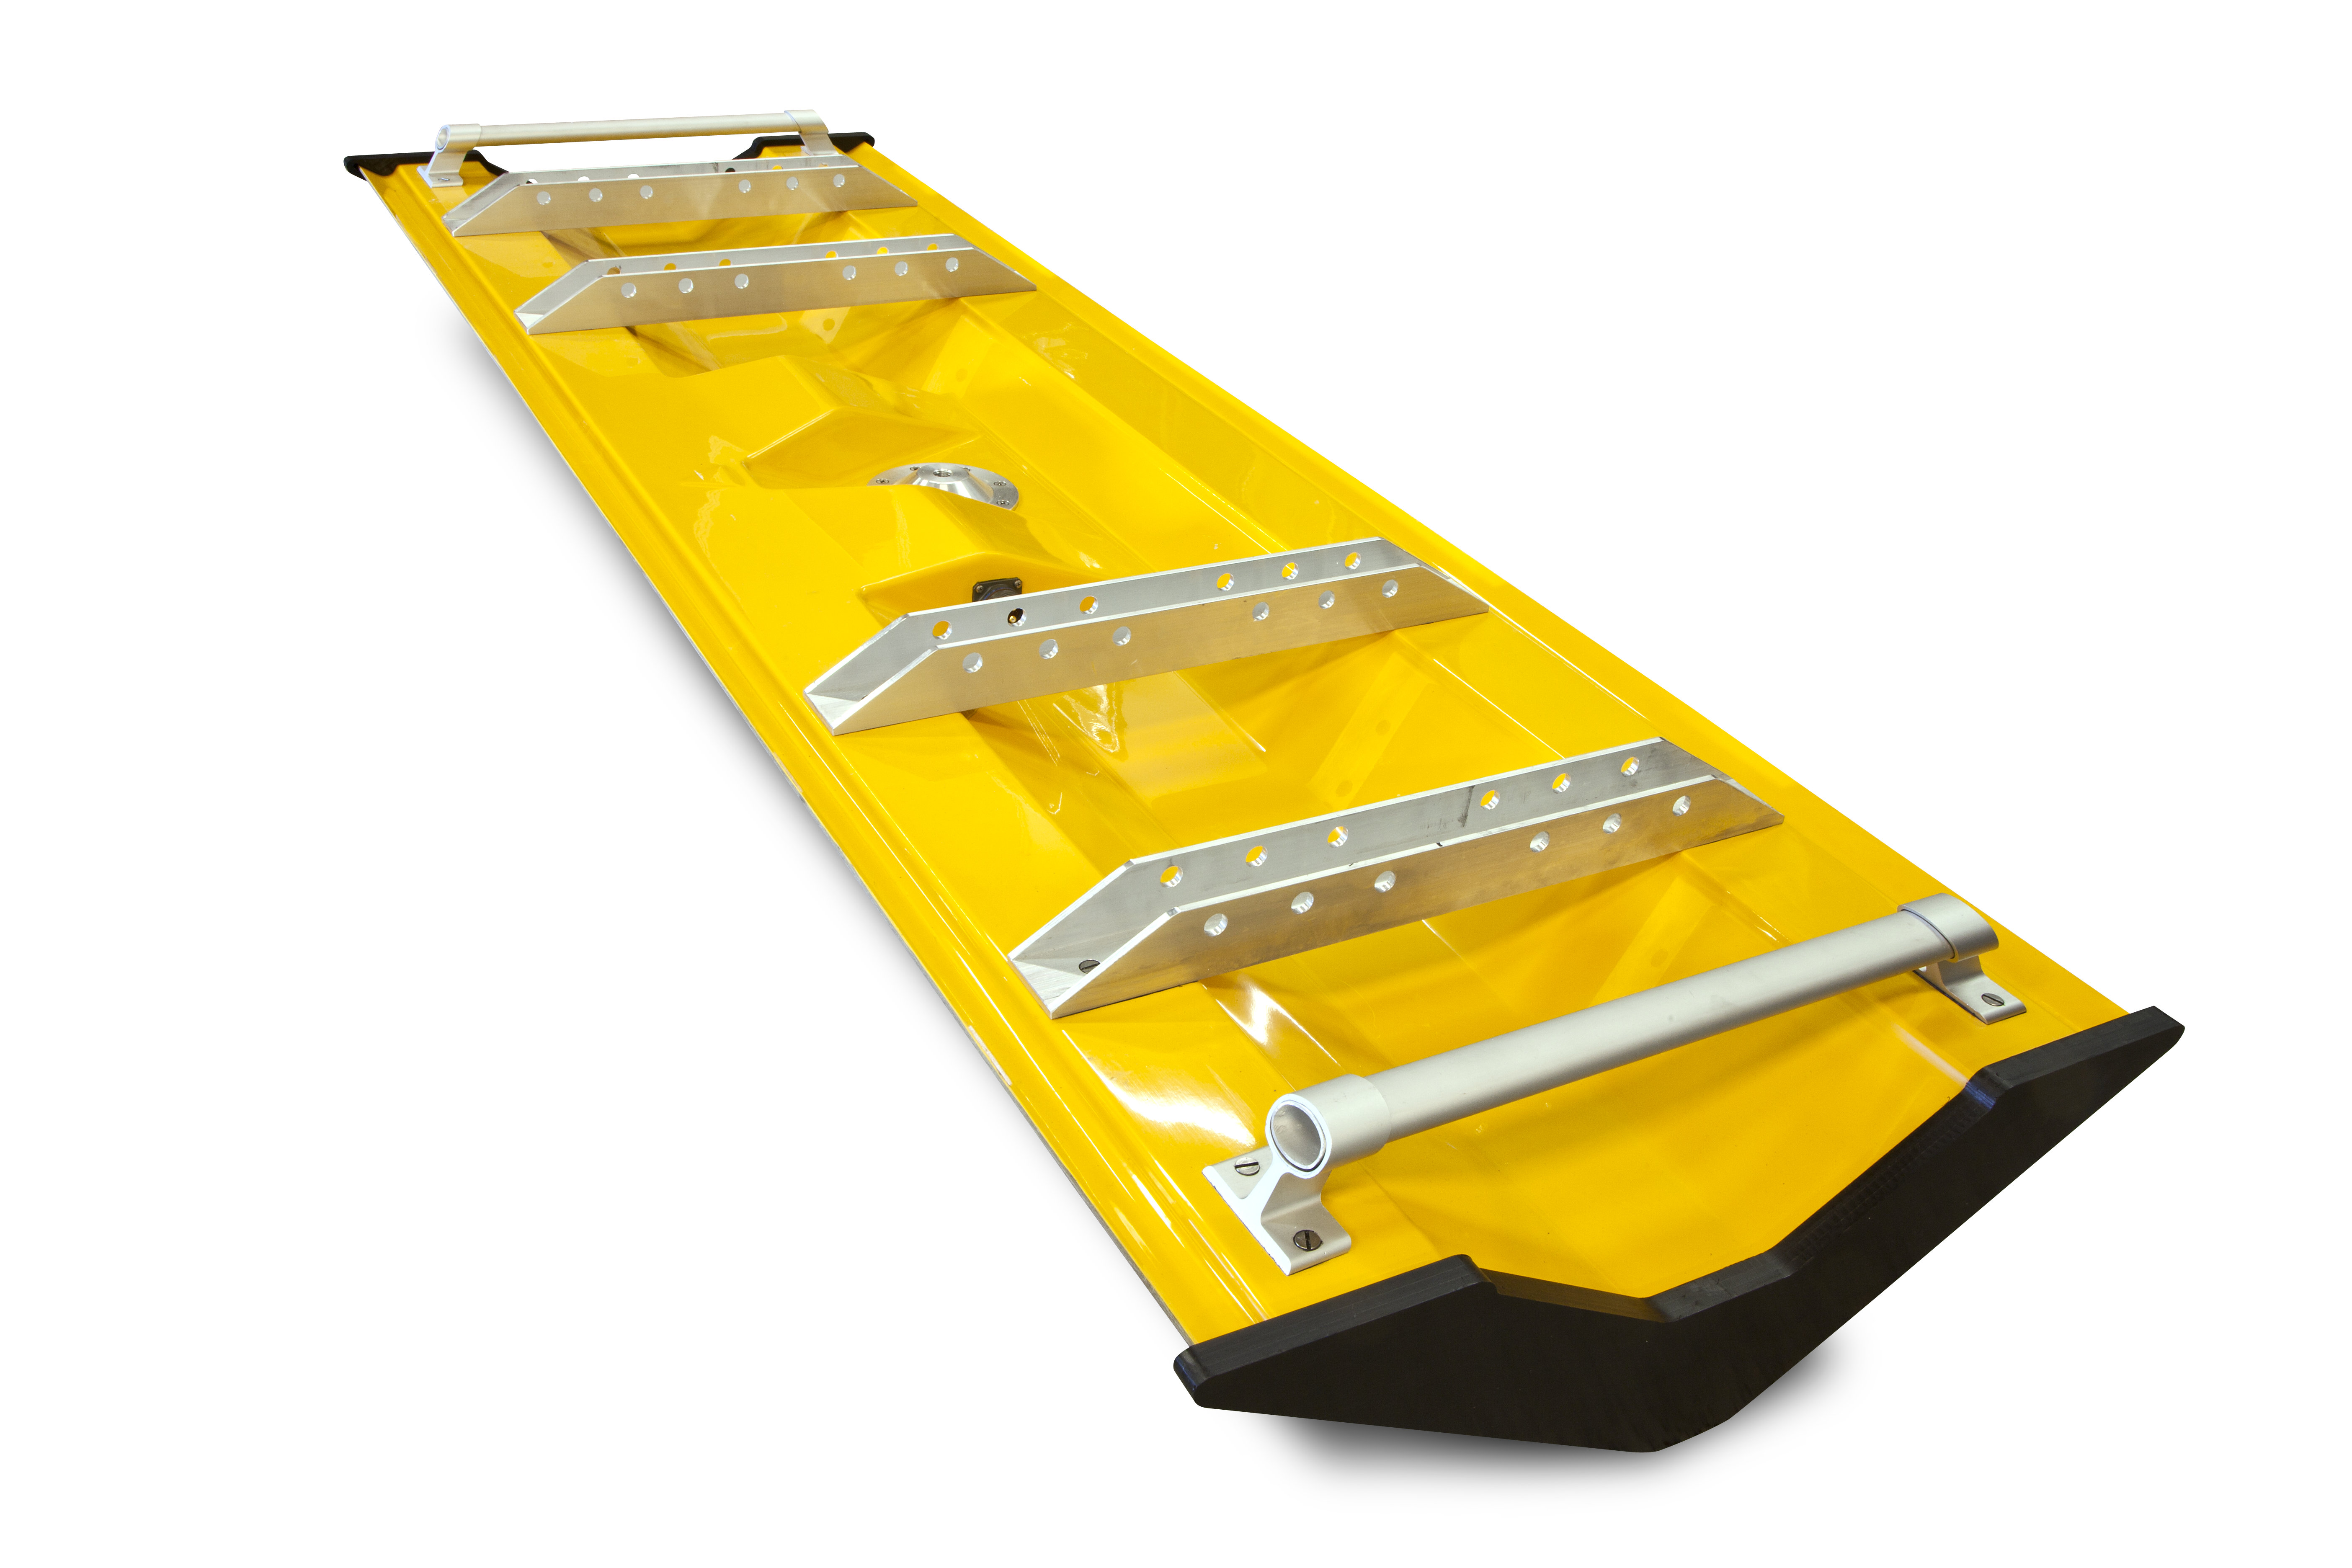
\includegraphics[width=0.8\textwidth]{2-Benchmarking/DX-Series-Antenna-Profile.jpg}
\caption{3D-RADAR DX Series GPR Antenna \parencite{3dradarDX}}
\figlabel{dxseries}
\end{figure}

\section{Multisensor Systems for Landmine Detection}
While traditional systems for landmine detection make use of a single sensor, the latest generation of systems attempt to combine multiple sensors. This allows for a broader range of threats to be detected, and at the same time increase detection accuracy.  

% There is no benchmark here so no point talking about it
%\paragraph{AN/PSS-14} The AN/PSS-14, formerly known as the Handheld Standoff Mine Detection System (HSTAMIDS), is the standard mine detector used by the US army since 2006 \parencite{L32012}. The system combines a ground penetrating radar with a metal detector and is designed to detect both anti-tank and anti-personnel mines. The wide-band GPR has a single transmit and two receive antennas, and forms the central part of the sensor head, while the metal detector coil sits around the GPR. Sensor fusion allows data from both sensors to be used in threat detection, which maximises probability of detection of the system while minimising the false alarm rate. In addition, the AN/PSS-14 system makes use of a real-time terrain model, which allows for optimal operation in varying soil conditions \parencite{L32012}. 

One such example is the Vallon Minehound, a commercially available handheld detector that combines a Vallon metal detector with a Cobham GPR \parencite{WM2016}. While the system is designed to find anti-tank and anti-personnel mines, it can also detect low metal content threats such as IEDs. 
%The metal detector employs pulse induction detection to find threats even in soils with a high mineral content, and can be used either independently or in conjunction with the GPR. 
%When used in conjunction, metallic clutter may be ignored, and non-metallic threats can be found. 
System performance in average soil condition allows for detection at depths up to 20 cm for anti-personnel and 40 cm for anti-tank mines, with an overall false alarm rate less than 25\% \parencite{daniels2005}.

Another system is being developed to allow demining and reclamation of vast swathes of currently unsafe land in rural Egypt, where remnants of World War II still pose a significant risk to local communities. The challenge of the Egyptian sands is that the frequently shifting ground surface means that mines are periodically uncovered or more deeply buried than when originally placed many decades ago \parencite{NATOnewsroom}. The system developed combines a highly sensitive metal detector, capable of recognising metallic objects buried at depths greater than a metre, with a GPR which is used to determine the shape and volume of objects located by the metal detector \parencite{NATOnewsroom}. This arrangement allows the detection of deep objects and a reduction in the rate of false positives, reducing the frequency of costly deep excavations of harmless shrapnel.


% There is no benchmark here, so no point talking about it
%\paragraph{ALIS} The Advanced Landmine Imaging System, or ALIS, is a Japanese system that can be integrated with an existing metal detector with minimum modification  \parencite{sato2005}. In addition to the audio output produced by the metal detector, ALIS produces a visual image that combines the metal detector signals with GPR images. The GPR used is a 1-3 GHz impulse radar system, and in order minimise the effect on the metal detector coils, it is mounted at the front of the system  \parencite{sato2005} The signals from both sensors are co-located through the use of a camera mounted on the system, which tracks the relative position of each one.


% Link to challenges in integration 

%The current challenges with landmine detection, including further elaboration of each signal processing methods are \textcolor{red}{reference literature review section}. 

\end{document}